\appendix
\section{Graph RAG Introduction}
\label{app:graph rags}
The Retrieval-Augmented Generation (RAG) system enhances large
language models (LLMs) by integrating external knowledge bases,
enabling real-time access to up-to-date information without retraininging. This approach addresses LLMs’ limitations in handling new
or domain-specific knowledge while reducing training costs and
mitigating the "illusion" problem, where models generate factually incorrect content. Traditional Naïve RAG achieves this by
converting external data into text chunks, vectorizing them, and
retrieving the most relevant segments for question answering. However, real-world knowledge often exists in graph structures, where
entities (nodes) and their relationships (edges) are key. This limitation has driven the evolution from text-based RAG to Graph RAG,
which leverages graph-structured knowledge for more accurate
and contextually rich retrieval and generation.

Graph RAG then proposes its Graph RAG solution, which
further performs entity extraction and relationship extraction operations on the text chunk partitioned by the traditional RAG, and
generates entity- and relationship-specific summaries as attributes
after extraction. After constructing a graph knowledge structure
consisting of nodes and edges, Graph RAG further runs community
discovery algorithms on the graph structure form summaries for
the communities, and reorders the summaries of the communities
as auxiliary contexts when answering questions. Such an approach,
when applied in practice, creates the problem of long data preparation time as well as limited scalability because of the need for
community discovery when constructing the graph structure.

Light RAG proposes a hierarchical context retrieval approach,
specifically, after constructing the knowledge of the graph structure, Light RAG does not further operate against the communities,
but rather, from the user’s question instead, Light RAG introduces
a dual-level retrieval paradigm that extracts entity-related keywords and relationship-related keywords from the user’s problem,
and directly retrieves the keywords. Entity keywords can be used
to solve more specific problems, while relationship keywords can
be used to solve more macroscopic conceptual problems, and Light
RAG integrates and rearranges the node and edge information
retrieved from the two hierarchical levels to form the final context.

Fast Graph RAG is an efficient graph retrieval framework optimized for large-scale application scenarios, which is designed to
improve the efficiency and accuracy of knowledge retrieval through
efficient graph construction operations and optimized retrieval
strategies. The framework introduces the PageRank algorithm to
reorder the retrieved nodes and edges to further enhance the relevance and reliability of the retrieval results. In addition, Fast Graph
RAG provides a graphical knowledge view that allows users to observe and navigate the retrieval process intuitively, which enhances
the interpretability and debuggability of the system.

% Graph Cot is a graph retrieval framework that incorporates
% the idea of chain of thought, which aims to solve the complex
% knowledge graph retrieval problem through a step-by-step retrieval
% strategy. The framework guides the retrieval process through an
% agent decomposes the retrieval task into multiple steps, and dynamically adjusts the retrieval strategy at each step. Specifically,
% each iteration of Graph Cot consists of three sub-steps: Reasoning,
% Interaction, and Execution. This process will continue until the
% LLM arrives at a final answer in the Reasoning step, which serves
% as the termination condition for the multiple rounds of step-by-step
% retrieval.

\section{Heat Maps}
\label{app:heatmaps}
\begin{figure}[t!]  % 使用 figure 环境，可以添加标题和编号
    \centering  % 图片居中
        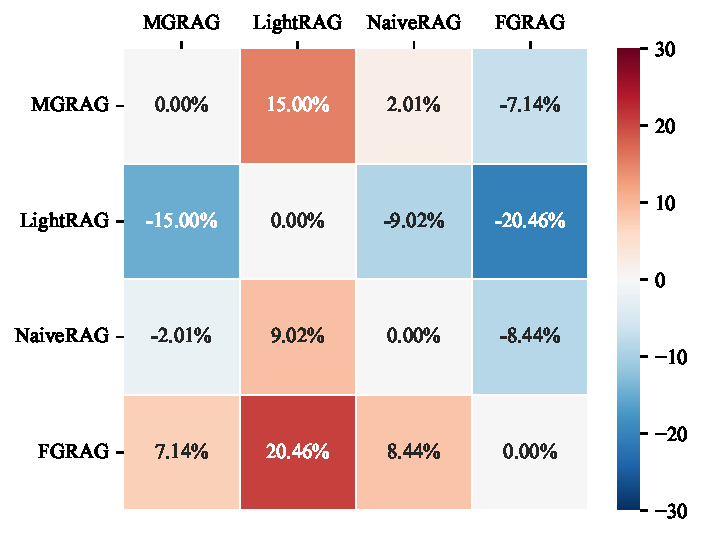
\includegraphics[width=0.33\textwidth]{pictures/mix-heatmap.pdf}  % 插入图片，设置宽度为文本宽度的 50%
    \caption{The performance comparison heatmap shows the relative win rate between model pairs over Mix dataset. A positive value indicates that the Row model outperforms the Column model and vice versa.}  % 添加图片标题
    \label{fig:heatmap-mix}  % 添加标签，用于引用
\end{figure}

\begin{figure}[h]  % 使用 figure 环境，可以添加标题和编号
    \centering  % 图片居中
        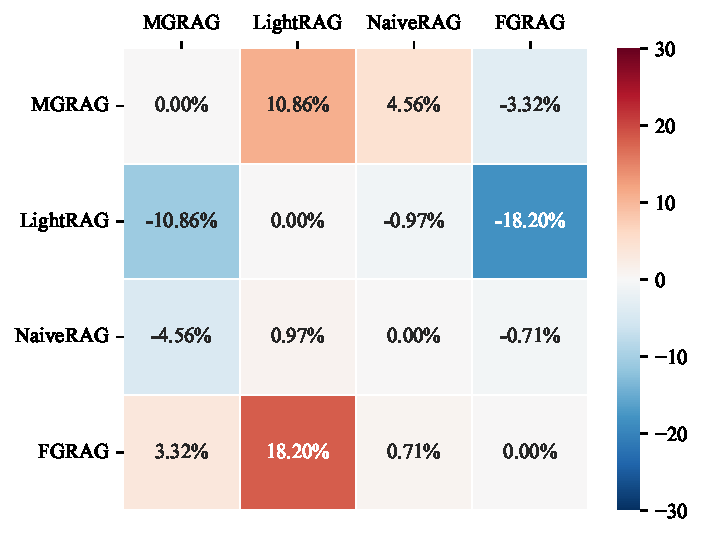
\includegraphics[width=0.33\textwidth]{pictures/agriculture-heatmap.pdf}  % 插入图片，设置宽度为文本宽度的 50%
    \caption{The performance comparison heatmap shows the relative win rate between model pairs over Agriculture dataset. A positive value indicates that the Row model outperforms the Column model and vice versa.}  % 添加图片标题
    \label{fig:heatmap-agriculture}  % 添加标签，用于引用
\end{figure}

\begin{figure}[h]  % 使用 figure 环境，可以添加标题和编号
    \centering  % 图片居中
        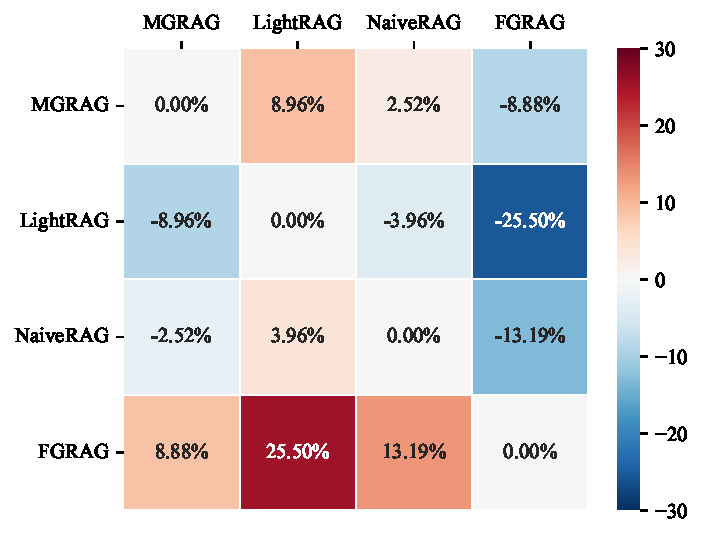
\includegraphics[width=0.33\textwidth]{pictures/music-heatmap.pdf}
    \caption{The performance comparison heatmap shows the relative win rate between model pairs over Music dataset. A positive value indicates that the Row model outperforms the Column model and vice versa.}  % 添加图片标题
    \label{fig:heatmap-music}  % 添加标签，用于引用
\end{figure}

This section shows the specific relative win rates on three datasets, and it can be seen that the distribution of relative win rates for the three plots is generally consistent with the mean plots shown in the paper, i.e., the relative win rates for the vast majority of comparisons are not particularly high, but there are a couple of exceptional values (e.g., FGRAG vs. LightRAG)

\section{Detailed Performance on Other Datasets}
\label{app:detailed}
\begin{figure*}[t!]  % 使用 figure 环境，可以添加标题和编号
    \centering  % 图片居中
    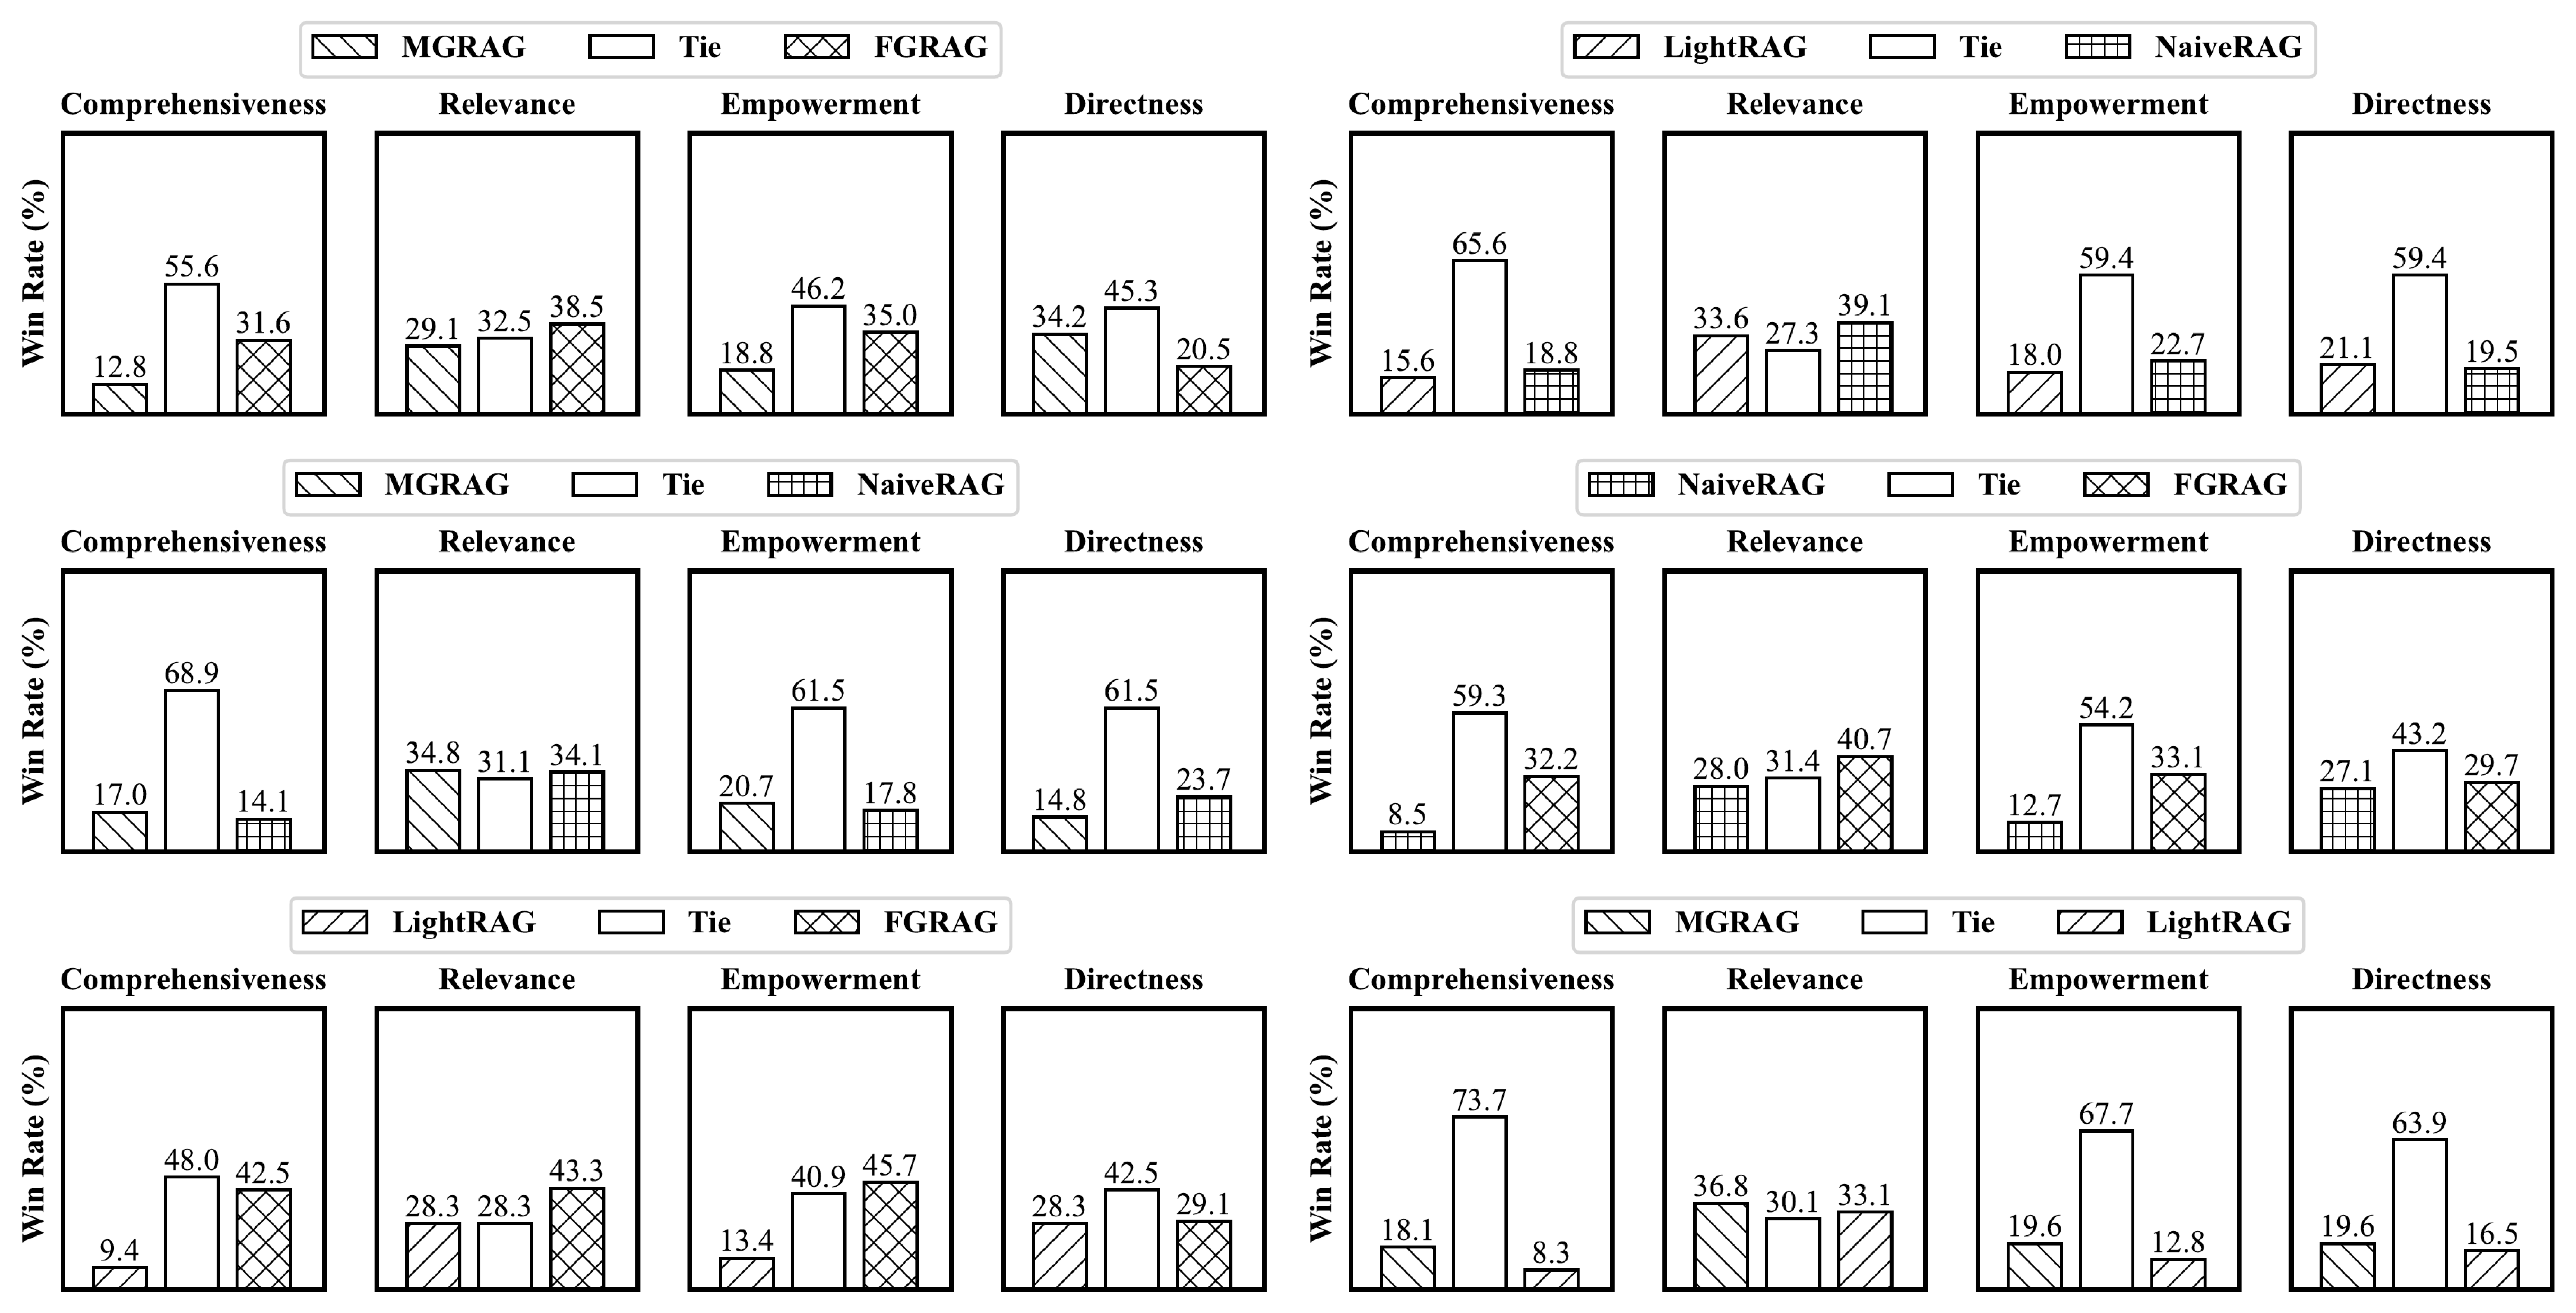
\includegraphics[width=0.99\textwidth]{pictures/agriculture-detail.pdf}  % 插入图片，设置宽度为文本宽度的 50%
    \vspace{-1.5em}
    \caption{Detailed win rate comparison across the four introduced aspects for model pairs under Agriculture dataset.}  % 添加图片标题
    \label{fig:detail-agriculture}  % 添加标签，用于引用
\end{figure*}
\begin{figure*}[t!]  % 使用 figure 环境，可以添加标题和编号
    \centering  % 图片居中
    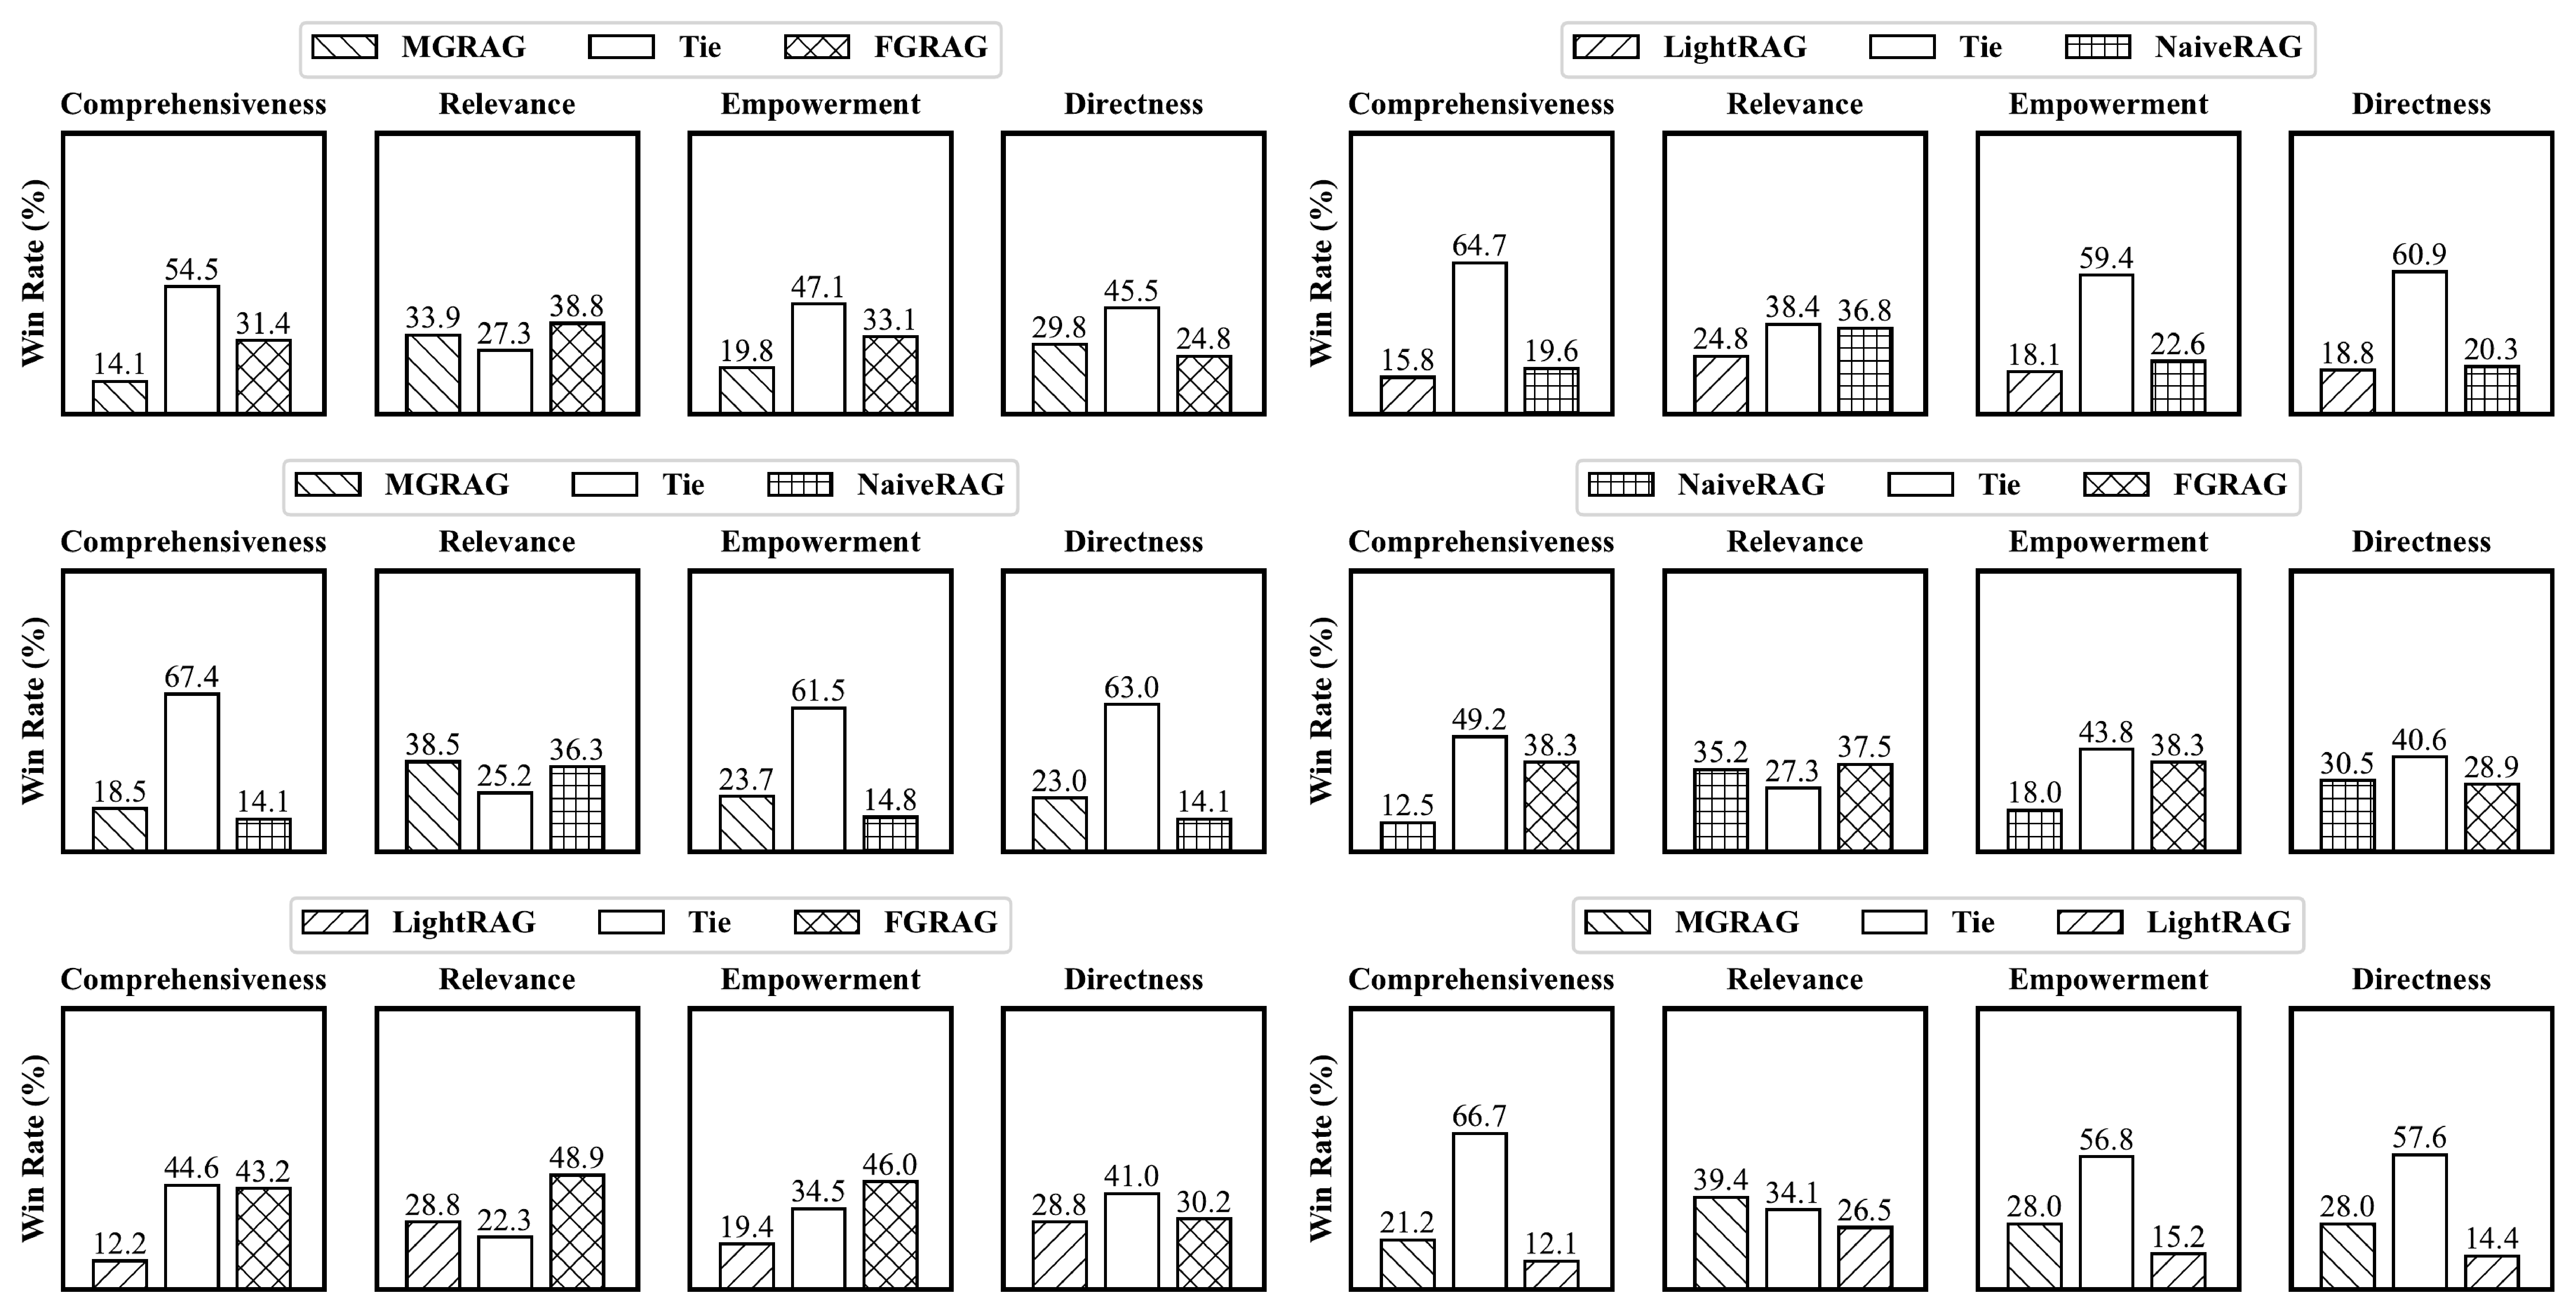
\includegraphics[width=0.99\textwidth]{pictures/mix-detail.pdf}  % 插入图片，设置宽度为文本宽度的 50%
    \vspace{-1.5em}
    \caption{Detailed win rate comparison across the four introduced aspects for model pairs under Mix dataset.}  % 添加图片标题
    \label{fig:detail-mix}  % 添加标签，用于引用
\end{figure*}

This section presents comparisons of specific aspects of the two datasets not included in the main text. The observations align with those in the main text, but the comparisons between LightRAG and NaiveRAG do not exhibit the same level of consistency as those between MGRAG and FGRAG. The comparative results between MGRAG and FGRAG remain valid, and many instances of ties can still be observed. We speculate that this discrepancy is primarily influenced by the size of the dataset. When the dataset is significantly larger, the superior comprehensiveness of LightRAG's answers becomes more apparent.

\renewcommand{\arraystretch}{2}
\begin{table*}
  \caption{Case Study}
  % \vspace{-0.5em}
  \label{tab: casestudy}
\begin{tabular}{|p{0.1\textwidth}|p{0.85\textwidth}|}
\hline
\textbf{Question} & \textbf{What school did Harry Potter attend?} \\
\hline
\textbf{Answer 1} & \# The School Harry Potter Attends:Harry Potter attends **Hogwarts School of Witchcraft and Wizardry**. This institution, often simply called **Hogwarts**, serves as the central educational setting within the Harry Potter series. \#\# Significance of Hogwarts Hogwarts is not just a school; it is a vital part of the narrative, providing a rich backdrop for magical education and diverse experiences for its students. The institution fosters learning in a variety of magical subjects, which play a crucial role in the development of Harry and his peers throughout the series. In summary, Hogwarts School of Witchcraft and Wizardry is integral to the story, shaping the characters and their journeys within the realm of magic. Harry Potter attends Hogwarts School of Witchcraft and Wizardry, a prestigious magical institution. It is the primary setting for his adventures and self-discovery. \\
\hline
\textbf{Answer 2} & \#\# Significance of Hogwarts Hogwarts is known for its strong educational framework. Students are sorted into four houses: Gryffindor, Hufflepuff, Ravenclaw, and Slytherin. The school provides comprehensive magical education and serves as a safe haven in troubled times.\#\# Harry's Experience At Hogwarts, Harry faces challenges, forms lasting friendships with Hermione Granger and Ron Weasley, and participates in magical adventures, including playing Quidditch as a Seeker for Gryffindor. These experiences shape his identity and give him a sense of belonging he lacks with the Dursleys. Overall, Hogwarts is crucial to Harry's growth as a young wizard. \\
\hline
\textbf{\parbox{0.1\textwidth}{Random \\ Select Judge}} & 
\parbox{0.85\textwidth}{
\vspace{0.3cm} 
Aspect 1:\\
Explanation: "Both answers provide detailed information about Hogwarts School of Witchcraft and Wizardry, covering its significance in the Harry Potter narrative. However, Answer 2 goes deeper into Harry's experiences at Hogwarts, including details about house sorting and personal challenges, while also addressing the educational framework and community aspects. Answer 1, though comprehensive, lacks the same level of detail concerning Harry's experiences." \\ Answer 1: 4, \textbf{Answer 2: 5}} \\

 & \parbox{0.85\textwidth}{
 \vspace{0.3cm} 
 Aspect 2: \\
 Explanation: Both answers directly address the question, identifying Hogwarts as the school Harry attends. They both remain relevant throughout, discussing its significance and how it impacts Harry. However, Answer 2 provides more context and richer details about Hogwarts and its relevance to the character, making it more aligned overall. \\
 Answer 1: 4, \textbf{Answer 2: 5}} \\

 & \parbox{0.85\textwidth}{
 \vspace{0.3cm} 
 Aspect 3:\\
 Explanation: Both answers help the reader understand the role of Hogwarts in Harry's life, but Answer 2 more effectively empowers the reader by detailing Harry's friendships and challenges, thereby enabling a deeper understanding of how the school influences his journey. Answer 1 offers a good overview but does not provide the same degree of insight into personal growth.\\
 Answer 1: 3, \textbf{Answer 2: 5}} \\

 & \parbox{0.85\textwidth}{
 \vspace{0.3cm} 
 Aspect 4: \\
 Explanation: Answer 1 is clear and direct in addressing the question but uses slightly more generalized language when discussing the significance of Hogwarts, whereas Answer 2 is exceptionally direct, offering specific details about Harry's school life, thus addressing the question with greater clarity. \\
 Answer 1: 4, \textbf{Answer 2: 5} \vspace{0.3cm} }\\
\hline
\textbf{Overall} & \parbox{0.85\textwidth}{
\vspace{0.3cm} 
Answer 1 Aspect 1: 3.75\\
Answer 1 Aspect 2: 4.25 \\
Answer 1 Aspect 3: 3.25\\
Answer 1 Aspect 4: 4.0 \\
Answer 1 Total: 15.25  \vspace{0.3cm}\\
Answer 2 Aspect 1: 5.0   \\
Answer 2 Aspect 2: 4.75 \\
Answer 2 Aspect 3: 5.0  \\
Answer 2 Aspect 4: 5.0 \\
\textbf{Answer 2 Total: 19.75}} \vspace{0.2cm} \\
 
\hline
\end{tabular}
\end{table*}

\section{Case Study}
\label{app:case study}
In this section, we provide an evaluation case to prove that our evaluation metric is efficient. The results are present in Table \ref{tab: casestudy}

As illustrated in the example provided, the evaluation system we proposed assigned scores to both answers to the same question from four distinct aspects. Upon analysis, it is evident that Answer 2 achieved higher scores across all dimensions. This superior performance can be attributed to the fact that Answer 2 not only encompassed the content of Answer 1 but also expanded upon it by incorporating a detailed description of Harry Potter's experiences at Hogwarts School of Witchcraft and Wizardry. This additional information rendered Answer 2 more comprehensive and contextually relevant to the question posed. Consequently, Answer 2 demonstrates greater utility in addressing the query, providing enhanced clarity and depth for the inquirer. This outcome underscores the importance of incorporating supplementary details that align with the thematic focus of the question, thereby elevating the overall quality of the response.

\section{Performance Across Different Question Types}
\label{app:questiontype}

In this section, we show the average win rates of different GraphRAG methods under different types of questions. 

% 可以看到，MGRAG在Node level问题上表现最佳，我们认为这是因为MGRAG产生的社区报告在面对几个实体时会显得非常精细，在有丰富信息量的同时没有那麽多冗余信息。FGRAG整体的表现可以概括为：subgraph level > edge level > node level。这也符合Graph RAG设计的初衷，即更好的解决复杂的需要对数据集有更全面理解的问题。我们观察了FGRAG检索的信息，发现其对node的信息概述略显简单，我们猜测这也是为什么其在node level上并没有展现出强大的优越性，同为类似设计的Graph RAG方法，Light RAG虽然在更复杂的问题上也展现出了一定能力提升，但是并没有显著优势。我们通过对其数据的观察猜测其有两方面原因，第一方面是每一个entity的信息量相对较大，并且还进行了一跳扩展，这使得检索到的信息噪声更大，另一方面是由于其不想FGRAG利用PageRank一样有一个很好的排序算法。

Our experimental results indicate that MGRAG achieves superior performance on node-level questions, which can be attributed to its ability to generate highly fine-grained community reports with minimal redundancy while maintaining rich information for a limited number of entities. In contrast, the overall performance of FGRAG follows a hierarchical ranking: subgraph level > edge level > node level. This aligns with its original design objective of addressing complex problems that require a comprehensive understanding of the dataset. Upon analyzing the information retrieved by FGRAG, we observed that its node-level summaries are comparatively less detailed, which may explain its relatively weaker performance at this level.

Additionally, Light RAG, a similarly designed Graph RAG approach, demonstrates limited advantages over other methods, despite showing marginal improvements on more complex questions. We believe that this is due to two factors: (1) the inclusion of extensive information from one-hop expansions, which introduces noise into the retrieved data, and (2) the lack of an effective ranking mechanism, such as the PageRank algorithm utilized by FGRAG, to prioritize relevant information. These observations provide insights into the strengths and limitations of different Graph RAG methodologies.

The overall performance of NaiveRAG exhibits an inverse trend compared to Graph RAG approaches, with significantly lower effectiveness on subgraph-level questions relative to node-level and edge-level questions. This aligns with its design, which relies on direct retrieval of fixed-length text segments for augmentation-a strategy that proves inadequate for addressing the complexity of subgraph-level questions. This limitation underscores the challenges of using simplistic retrieval methods for questions requiring broader contextual understanding.

\begin{figure}[b]  % 使用 figure 环境，可以添加标题和编号
    \centering  % 图片居中
        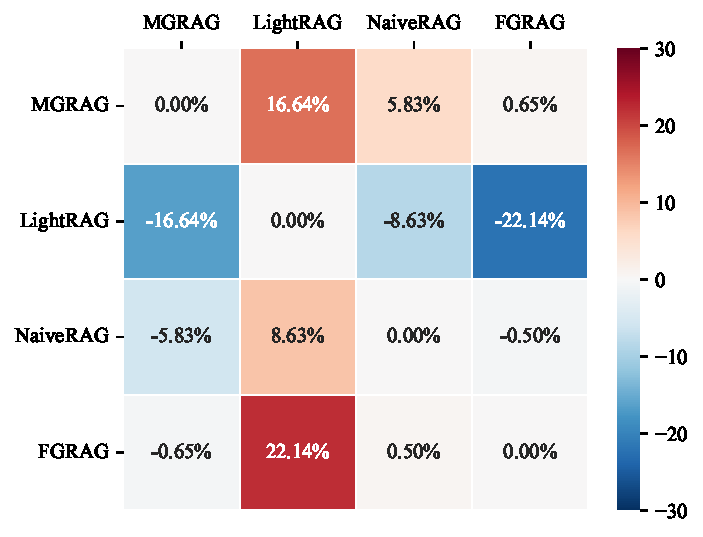
\includegraphics[width=0.35\textwidth]{pictures/mix-agriculture-music-question-1-average-heatmap.pdf}  % 插入图片，设置宽度为文本宽度的 50%
    \caption{The average win rate comparison across the four baseline model pairs evaluated on node-level questions under three datasets (Mix, Agriculture, and Music).}  % 添加图片标题
    \label{fig:heatmap-mix}  % 添加标签，用于引用
\end{figure}

\begin{figure}[b]  % 使用 figure 环境，可以添加标题和编号
    \centering  % 图片居中
        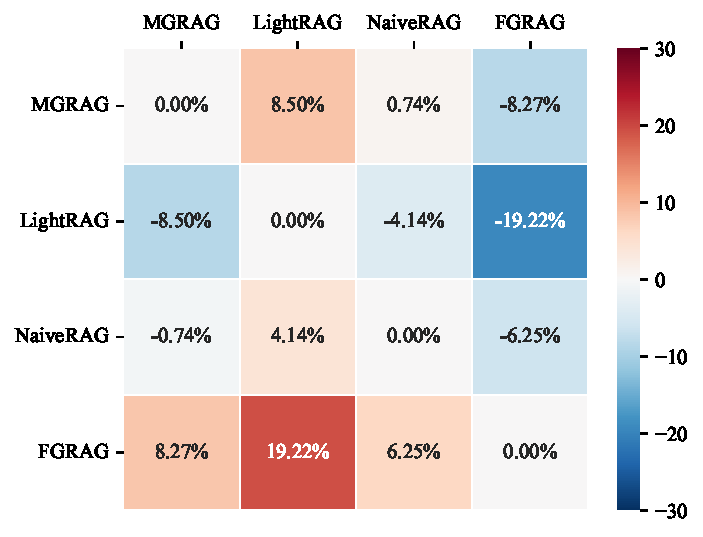
\includegraphics[width=0.35\textwidth]{pictures/mix-agriculture-music-question-2-average-heatmap.pdf}  % 插入图片，设置宽度为文本宽度的 50%
    \caption{The average win rate comparison across the four baseline model pairs evaluated on edge-level questions under three datasets (Mix, Agriculture, and Music).}  % 添加图片标题
    \label{fig:heatmap-agriculture}  % 添加标签，用于引用
\end{figure}

\begin{figure}[b]  % 使用 figure 环境，可以添加标题和编号
    \centering  % 图片居中
        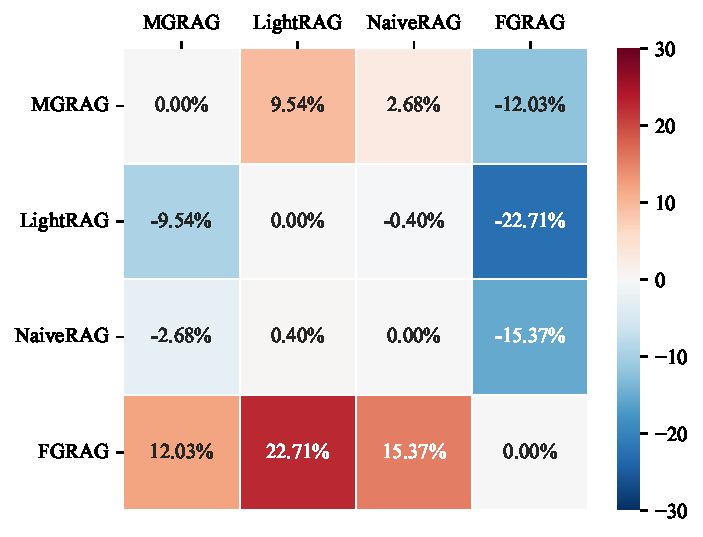
\includegraphics[width=0.35\textwidth]{pictures/mix-agriculture-music-question-3-average-heatmap.pdf}
    \caption{The average win rate comparison across the four baseline model pairs evaluated on subgraph-level questions under three datasets (Mix, Agriculture, and Music).}  % 添加图片标题
    \label{fig:heatmap-music}  % 添加标签，用于引用
\end{figure}